\documentclass[%
aip,
jmp,
reprint,
floatfix
]{revtex4-1}

\usepackage{graphicx}% Include figure files
\usepackage{dcolumn}% Align table columns on decimal point
\usepackage{bm}% bold math
\usepackage{float}
\usepackage{siunitx}
\usepackage{hyperref}
\usepackage{listings}
%\usepackage[style=phys]{biblatex}
%\addbibresource{refs.bib}
\usepackage{ gensymb }
%\usepackage[mathlines]{lineno}% Enable numbering of text and display math
%\linenumbers\relax % Commence numbering lines
\usepackage{color}

\definecolor{dkgreen}{rgb}{0,0.6,0}
\definecolor{gray}{rgb}{0.5,0.5,0.5}
\definecolor{mauve}{rgb}{0.58,0,0.82}

\lstset{
	frame=single, 
	language=Python, 
	columns=flexible,
	basicstyle={\footnotesize\ttfamily},
	keywordstyle=\color{blue},
	commentstyle=\color{dkgreen},
	stringstyle=\color{red},
	title=\lstname
}


\renewcommand{\arraystretch}{1.3} % Changes the height of tables
\DeclareSIUnit\year{yr}
\DeclareSIUnit\parsec{pc}



\begin{document}

	\title[Photometry of M39]{Differential Photometry of M39}

	\author{Lucas, Miles}
	\author{Brandon, John}
	\affiliation{Iowa State University Department of Physics and Astronomy}

	\date{\today}


% Write here a short abstract (1 paragraph) describing what you achieved in this lab.

	\begin{abstract}
	We used differential photometry to determine magnitudes of four objects in M39 using two foreground stars as references. We could only process three of the objects of interest due to poor image data for the other objects. The magnitudes were as follows: BD+47 3447, V=\SI{10.189\pm0.019}{}, B=\SI{10.394\pm0.056}{}, HD 205085  V=\SI{7.9696\pm0.0075}{} B=\SI{8.0264\pm0.0016}{}, and BD+47 3453, V=\SI{9.540\pm.010}{}, B=\SI{9.669\pm0.024}{}. The reference stars we used were BD+47 3454, V=\SI{8.917}{}, B=\SI{9.028}{} and HD 205073, V=\SI{7.845}{}, B=\SI{7.870}{}. Our magnitudes agree with other papers on M39 and our precision is around one-hundredth of a magnitude. We noted our brighter stars have less error, generally.

	\end{abstract}

	\maketitle
%________________________________________________________________________

%	Write here a summary of the goals of this lab. Be brief – do not exceed the end of the first page.

	\section{Introduction}

	This lab seeks to determine the V and B magnitudes of four objects in M39, an open galactic cluster. M39 contains around 30 stars of various brightness and is about \ang{9} from Deneb ($\alpha$ Cyg). 
	
	To determine the magnitudes of our objects, we used differential photometry. This process uses the simplicity of having two objects taken in the same image, through the same filter, through the same optical path, and exposed for the same amount of time to determine
	\begin{equation}
		m_{tar} = m_{ref} + m_{diff}
		\label{eqn:diff}
	\end{equation}
	
	The way an imaging program does this is by determining the instrumental magnitudes and then comparing them to the reference magnitudes. 
	\begin{equation}
	 	m_{inst} = -2.5 \log_{10}(S-B)
	 	\label{eqn:inst}
	\end{equation}
	where $S$ is the sum of all the pixel values in a given aperture and $B$ is the sum of all the pixel values of some background section, usually an annulus. The way AstroImageJ calculates these sums is dependent on more complex equations that parameterize the electron gain of the CCD and can do more image processing prior to integrating the pixel values. These extra parameters allow for determining the error of the instrumental magnitude.
	
	After the instrumental magnitude of a reference star is found, we can determine the magnitude correction value by combining \autoref{eqn:diff} and \autoref{eqn:inst}.
	
	\begin{equation}
		m_{corr} = m_{ref} - m_{inst}
		\label{eqn:corrected}
	\end{equation}
	and finally we can find the magnitude of any target star with 
	\begin{equation}
		m_{tar} = m_{inst} + m_{corr}
		\label{eqn:final}
	\end{equation}
	
	We used a weigthed average and standard deviation to report our numbers, with weight equal to the inverse error squared.
	\begin{equation}
	 	\bar{x}_w = \frac{\sum_i{x_i/\sigma_i^2}}{\sum_i{1/\sigma_i^2}}
	 	\label{eqn:wa}
	\end{equation}
	\begin{equation}
	\sigma_w = \sqrt{\frac{1}{n-1} \sum{(x_i -\bar{x}_w)^2}}
	\label{eqn:ws}
	\end{equation}
	

%________________________________________________________________________

%	Describe your telescope and camera setup. For the first lab you should describe the setup in more details. Subsequent labs can refer to the procedure described in the first lab, and focus more on the data acquisition itself. Important details to write include: which stars have been observed, which filters were used (BVI), what exposure times and what calibration procedures have been followed (e.g., dark frames acquisition, photometric standards observed, etc.). Mention also the observing conditions (weather, moon presence, temperature, etc.). You should include the observing log appendix A (a table or a scan of a hardcopy). This section can be as long as necessary, but you should strive for brevity (you can refer to the lab guide to avoid repeating all steps, but make sure you explain anything you did differently, problems encountered, etc.). Use tables to summarize information clearly.

	\section{Data Acquisition and Setup}
	Observations were made on \date{06 September 2017} at the Zaffarano Hall observation deck in Ames, Iowa (\ang{-93.64734}, \ang{42.02996}, \SI{342}{\meter}). The night was mostly clear and the ambient temperature was around \SI{12}{\degreeCelsius}. The moon was full that night which caused higher than usual lunar presence. Observations were made using a Meade 8" reflector telescope with an SBIG ST-402ME CCD camera with internal V, B, and I filters. 
	
	Setting up the telescope was the same as previous observations made with the 8" Meade telescope at Zaffarano Hall. An obstacle we faced with alignment and slewing was the misalignment of our sight by a significant amount. To combat this, we shined a laser through the eyepiece to roughly show the target of the main mirror.
	
	We took 15 frames of data at \SI{13}{\second} at two locations in the sky. Of those 15, 5 were with photometric V, 5 were with photometric B, and 5 were dark frames. The first target contained two M39 objects (BD+47 3452 and HD 205172), however this data was deleted by accident and was not used for analysis. The second target contained objects BD+47 3447, HD 205085, BD+47 3453, and BD+47 3458, all of which are recorded in \autoref{table:log}. Of these images, another issue we encountered was centering the images as the telescope shifted according to its tracking movements. Because of this, a few of the images do not contain a clear view of BD+47 3458.
	
	\begin{figure}[]
		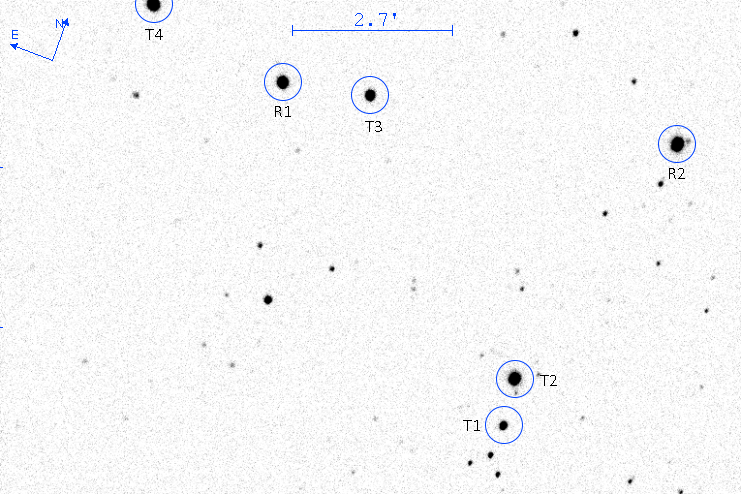
\includegraphics[width=\linewidth]{figs/M39_map.png}
		\caption{Map showing the celestial direction, target stars, and reference stars. The names of the objects above are in \autoref{table:phot}.}
		\label{fig:map}
			
	\end{figure}

%________________________________________________________________________

%Describe what you did to analyze the data. For the first lab this section will be minimal. For subsequent labs you should describe in detail the steps you did to analyze the data.  If applicable you can attach the code you used to analyze the data in Appendix B (either a log of your IDL section, or the code of any scripts you wrote). You can also attach screenshots of your computer session if it helps your discussion. Include tables of raw data in this section. The goal of this section is to describe unambiguously what you did to derive your final images and measured quantities from the raw data. Again be brief but complete (use as much space as you need).
	\section{Data Analysis}
	Our data analysis involved preparing our science images and performing differential photometry on them. To prepare our images we created a median dark frame in AstroImageJ for our only exposure time, \SI{13}{\second}. We then subtracted this frame from each science image to filter out systematic noise from our CCD. These images were then grouped into two stacks, one for each photometric filter.
	
	We used AstroImageJ to process each stack using multi-aperture photometry. Our reported electronic gain was \SI{1.49}{\elementarycharge\per{ADU}}. AstroImageJ processes the stack of images in a way that allows for quick aperture placement. An aperture can be placed on each star of interest in an image and AstroImageJ allows placing target stars and reference stars, where the reference stars have predetermined magnitudes.
	
	After placing the apertures for one image in the stack we move forward in the stack and by choosing the same initial aperture AstroImageJ will place the remaining apertures automatically. The reference magnitudes are shown in \autoref{table:ref}. After each aperture has been placed on each image in the stack and the reference star magnitudes have been set, AstroImageJ will do the photometry and creates a measurement table with the results. The full results are shown in \autoref{sec:res}. The skymap for the target and reference stars is shown in \autoref{fig:map}.

	\begin{table}[ht]
		\centering
		\caption{Reference Stars}
		\begin{tabular*}{0.7\linewidth}{@{\extracolsep{\fill}}rlrr}
			\hline
			Object & Name       &        V Mag &        B Mag \\ \hline\hline
			    R1 & BD+47 3454 & \SI{8.917}{} & \SI{9.028}{} \\
			    R2 & HD 205073  & \SI{7.845}{} & \SI{7.870}{} \\ \hline
		\end{tabular*}
		\label{table:ref}
	\end{table}

%________________________________________________________________________

%	Describe in detail the results you obtained from the quantitative analysis of your data, as explained in the lab guide.
	\section{Results}

	The table of the results from AstroImageJ are in \autoref{sec:res} and the results calculated using \autoref{eqn:wa} and \autoref{eqn:ws} are in \autoref{table:phot}. We do not report a magnitude for BD+47 3458 because of issues with the photometry. The star had drifted out of frame for some of the images and therefore the instrumental magnitude was not correct. Also, the star moved due to telescope drift and the amount of the star cut off was inconsistent which caused a large variance in the pixel value counts. 

	\begin{table}[ht]
		\centering
		\caption{Photometry Results}
		\begin{tabular*}{0.9\linewidth}{@{\extracolsep{\fill}}rlrr}
			\hline
			Object & Name       &                  V Mag &                  B Mag \\ \hline\hline
			    T1 & BD+47 3447 &  \SI{10.189\pm0.019}{} &  \SI{10.394\pm0.056}{} \\
			    T2 & HD 205085  & \SI{7.9696\pm0.0075}{} & \SI{8.0264\pm0.0016}{} \\
			    T3 & BD+47 3453 &    \SI{9.540\pm.010}{} &   \SI{9.669\pm0.024}{} \\
			    T4 & BD+47 3458 &                     NA &                     NA \\ \hline
		\end{tabular*}
		\label{table:phot}
	\end{table}

%________________________________________________________________________

%	Add here anything else you want to say, and summarize your results. This section should be very brief, not more than a couple of paragraphs
	\section{Conclusions}
	
	Although we encountered issues with framing the images and accidentally deleting half of our data, we are satisfied with the results of the differential photometry. A quick comparison to the magnitudes reported by other papers shows that we are mostly accurate and our process was effective given our equipment. The precision of our photometry as also reasonable. We are happy to see that we can generally be precise to the hundredth of a magnitude. We also noted that the brighter the object the less error we had.

%________________________________________________________________________

	\section*{Acknowledgments}

	Thank you to Dr. Charles Kerton and Brandon Marshall for their guidance and assistance in this work.

%	\printbibliography


%________________________________________________________________________

	\onecolumngrid
	\appendix
	\section{Observation Log}

	\begin{table}[H]
		\centering
		\caption{Observed 06 September 2017 by Miles Lucas and John Brandon}
\begin{tabular}{clclcccl}
	\hline
	Time  & File                   & N Frames & Object                                     & Filter &     Exposure     &       Camera Temp.        & Notes       \\ \hline\hline
	21:39 & M39\_2\_V\_13s\_       &    5     & M39 Objects x1, x4, x7, and x9; stars E, D &   V    & \SI{13}{\second} & \SI{5.33}{\degreeCelsius} &             \\
	21:41 & M39\_2\_V\_13s\_dark\_ &    5     & M39 Objects x1, x4, x7, and x9; stars E, D &   V    & \SI{13}{\second} & \SI{5.33}{\degreeCelsius} & Dark frames \\
	21:43 & M39\_2\_B\_13s\_       &    5     & M39 Objects x1, x4, x7, and x9; stars E, D &   B    & \SI{13}{\second} & \SI{5.33}{\degreeCelsius} &             \\ \hline
\end{tabular}

		\label{table:log}
	\end{table}
%________________________________________________________________________

	\section{Photometry Results} \label{sec:res}
	
	\begin{table}[H]
		\centering
		\caption{Full results from AstroImageJ multi-aperture differential photometry for the photometric V filtered images}

\begin{tabular}{l|rr|rr|rr|rr|rr|rr}
	\hline
	Slice &    T1 Mag &   T1 Err &   T2 Mag &   T2 Err &   T3 Mag &   T3 Err &    T4 Mag &   T4 Err & R1 Mag &   R1 Err & R2 Mag &   R2 Err \\ \hline\hline
	1     &  10.18609 & 0.176984 & 7.960098 & 0.037337 & 9.537899 &  0.10435 &  8.716391 & 0.055953 &  8.917 & 0.061367 &  7.845 & 0.025834 \\
	2     & 10.193105 & 0.187644 & 7.973817 &  0.04062 & 9.537579 & 0.111398 &  8.786726 &  0.06126 &  8.917 &   0.0653 &  7.845 &  0.02774 \\
	3     & 10.195668 & 0.191079 & 7.968483 & 0.041178 & 9.529998 & 0.112293 &  9.008232 & 0.071347 &  8.917 & 0.066747 &  7.845 & 0.028051 \\
	4     & 10.220418 & 0.200807 & 7.963982 & 0.042037 & 9.557328 & 0.116375 &  9.249187 & 0.086958 &  8.917 &  0.06898 &  7.845 & 0.028695 \\
	5     & 10.169891 &  0.14342 & 7.978648 &  0.03339 & 9.537594 & 0.086798 & 10.330707 & 0.155808 &  8.917 & 0.051375 &  7.845 & 0.022805 \\ \hline
\end{tabular}
		\label{table:fullresv}
	\end{table}

	\begin{table}[H]
		\centering
		\caption{Full results from AstroImageJ multi-aperture differential photometry for the photometric B filtered images}
\begin{tabular}{l|rr|rr|rr|rr|rr}
	\hline
	Slice &    T1 Mag &   T1 Err &   T2 Mag &   T2 Err &   T3 Mag &   T3 Err & R1 Mag &   R1 Err & R2 Mag &   R2 Err \\ \hline\hline
	1     & 10.374302 & 0.058418 & 8.028253 & 0.019926 & 9.661362 & 0.038906 &  9.028 & 0.025439 &   7.87 & 0.014405 \\
	2     & 10.398856 & 0.072556 & 8.024075 & 0.023852 &  9.66782 & 0.047418 &  9.028 & 0.030662 &   7.87 & 0.017282 \\
	3     & 10.467363 & 0.175167 & 8.026245 & 0.033794 & 9.702747 & 0.094185 &  9.028 & 0.053192 &   7.87 & 0.023198 \\
	4     & 10.423689 & 0.190297 & 8.026522 & 0.036299 & 9.665717 & 0.103558 &  9.028 & 0.058534 &   7.87 & 0.024633 \\
	5     & 10.470166 & 0.211676 & 8.025427 & 0.038635 & 9.701385 & 0.114719 &  9.028 & 0.062982 &   7.87 &  0.02621 \\ \hline
\end{tabular}
		\label{table:fullresb}
	\end{table}


\end{document}
